\documentclass{article}


\usepackage{arxiv}

\usepackage[utf8]{inputenc} % allow utf-8 input
\usepackage[T1]{fontenc}    % use 8-bit T1 fonts
\usepackage{hyperref}       % hyperlinks
\usepackage{url}            % simple URL typesetting
\usepackage{booktabs}       % professional-quality tables
\usepackage{amsfonts}       % blackboard math symbols
\usepackage{nicefrac}       % compact symbols for 1/2, etc.
\usepackage{microtype}      % microtypography
\usepackage{mathtools}

\usepackage{graphicx}
\graphicspath{ {./images/} }

\title{DroneNet: using drone swarms for autonomous search and rescue}


\author{
  Jacky Zhao
  St. George's School\\
  Vancouver, CA\\
  \texttt{j.zhao2k19@gmail.com} \\
}

\begin{document}
\maketitle

\begin{abstract}
\texttt{
Current search and rescue methods are very reliant on global communication methods like GPS or a central control unit. This limits the range and efficiency of search and rescue operations. A decentralized drone swarm would alleviate these problems by having a theoretically infinite range given number of drones. So far, we have designed and assembled the first drone using 3D printed components and ordered parts, built the recognition network by retraining a YOLOv3 model on the KITTI dataset. The next component would be to implement the decentralized autopilot using a Deep Q-learning Agent or another reinforcement learning algorithm to output velocity deltas.
} \\
\end{abstract}


\section{Introduction}
Search and rescue (SAR) operations are some of the most important in the world, saving thousands of lives each year. However, SAR operations are severely hampered by the 'searching' aspect of SAR. THis is due to several factors, namely 1. speed of the operation, and 2. accuracy of detection. Firstly, many, if not most, SAR operations are conducted on foot or via helicopter. However, while on-foot operations are more accurate, they lack the speed to be very effective. Helicopter operations, on the other hand, are fast but are often prone to low accuracy. There have been many efforts to address this lack of a better solution, including proposals to use OpenCV and neural networks in drones for improved performance in the human-identification process. However, this improvement is still marginal as only one drone is being used at a time. Institutions such as MIT have proposed solutions which involve controlling a drone swarm for increased efficiency. Interestingly, there has been no published attempt at completing a project which involves creating both the human-detection and drone swarm management algorithms.

\section{Proposal}
\label{sec:headings}
We propose a novel end-to-end algorithm for controlling drone swarms for autonomous search and rescue. This algorithms would be able to,

\begin{enumerate}
  \item Efficiently navigate a 3D search space,
  \item Effectively communicate between an undetermined amount of drones and transfer data (location, images),
  \item Detect and identify humans
\end{enumerate}

As this task is extremely difficult, we plan to tackle this task in multiple stages. In the first stage, we plan to create a singular functioning drone which is able to navigate a 2D air space above a clear area, and efficiently find a human.

\subsection{Hardware}
\subsubsection{Frame}
The physical frame of the drone is a modified build of the Firefly 1504 Drone. The mainframe is modified by first expanding the width to be able to fit the battery. Bumper\_v2\_f.stl and 2x side.stld is printed with 50\% infill. Lower\_plate\_V2.stl, Top\_plate\_front\_3mm.stl, and Top\_plate\_rear\_3mm.stl are printed with 25\% infill. Arms are 100mm segments of Carbon Fiber tube with a radius of 6mm. Holes and screws were drilled and assembled as according to the documentation of the Firefly.

\subsubsection{Cost and Equipment Breakdown}
The breakdown of the price and weight data for the construction of the first drone is listed below.
\begin{table}[h!]
\centering
\begin{tabular}{|l|l|l|l|}
\hline
Quantity & Item                                    & Total Weight (g) & Price    \\ \hline
1x       & 3D Printed Frame                        & 50.0g            & N/A      \\ \hline
1x       & 1300mAh 4S 45C LiPo Battery             & 165.0g           & \$19.10  \\ \hline
4x       & 20A 2-4S ESC                            & 28.0g            & \$50.68  \\ \hline
1x       & HobbyKing Lite Power Distribution Board & 19.3g            & \$4.13   \\ \hline
4x       & 100mm x 6mm Carbon Fiber Tubes          & 45.2g            & \$7.99   \\ \hline
1x       & PXFMini Power Module                    & 50.0g            & \$44.94  \\ \hline
1x       & PXFMini                                 & 15.0g            & \$103.36 \\ \hline
4x       & EMAX RS2205 Brushless Motor             & 120.0g           & \$39.96  \\ \hline
4x       & GEMFAN 5045 GRP 3-BLADE Propellers      & 21.2g            & \$8.76   \\ \hline
1x       & Pi Zero W                               & 9.0g             & \$5.00   \\ \hline
1x       & Pi Camera v1 5MP                        & 18.1g            & \$14.99  \\ \hline
N/A      & Misc. wires, bolts, and nuts            & 20.0g            & N/A      \\ \hline
Totals   & N/A                                     & 560.8g           & \$298.91 \\ \hline
\end{tabular}
\caption{Price and Weight Breakdown}
\end{table}

\subsubsection{Flight}
In calculating the thrust required, we consider that the drone will not be used for racing. As a result, a thrust to weight ratio of 4:1 works well. Using the weight of the drone calculated in 2.1.2, we get a thrust requirement of 2.43kg. Dividing this by the 4 motors, we require 560g of thrust per motor. we decided on using the GEMFAN 5045 propellers (5" diameter, 4.5" pitch). This allows the drone to achieve a thrust of roughly 560g per motor at only 13A draw or 52A total.

\begin{table}[h!]
\centering
\begin{tabular}{|l|l|l|l|}
\hline
Current (A) & Thrust (g) & Efficiency (g/W) & Speed (RPM) \\ \hline
1           & 76         & 4.75             & 7220        \\ \hline
3           & 183        & 3.81             & 10790       \\ \hline
5           & 282        & 3.54             & 13030       \\ \hline
7           & 352        & 3.10             & 14720       \\ \hline
9           & 426        & 2.93             & 16180       \\ \hline
11          & 497        & 2.82             & 17150       \\ \hline
13          & 560        & 2.69             & 18460       \\ \hline
15          & 628        & 2.62             & 19270       \\ \hline
...         & ...        & ...              & ...         \\ \hline
27          & 997        & 2.28             & 23920       \\ \hline
30          & 1024       & 2.14             & 24560       \\ \hline
\end{tabular}
\caption{Thrust Table for RS2205-2300KV @ 16.8V with GF5045BN}
\end{table}

As such, we needed to choose a battery that would allow reasonable flight time given our 52A draw. We can use the Maximum Recommended Current Draw function which is as follows
\begin{equation}
I_{max} = Capacity_{Ah} \cdot C Rating
\end{equation}

For this project, a 1300mAh 4S 45C LiPo Battery was used.

\[
I_{max} = 1.3Ah \cdot 4C = 58.5A
\]

This max current is greater than the maximum theoretical usage, thus, this battery is safe to use. Using this information, we can calculate the theoretical maximum flight time. To keep the drone in the air, we require approximately thrust equal to the weight of the drone (560g). This translates to roughly $140g$ of thrust per motor. we assume that the capacity is only 80\% effective, meaning $1.04Ah$ is available. We can then convert to minutes by multiplying by $h/60min$ and dividing by the current draw of $3A$. This attains a total flight time of 20.8 minutes.

\subsubsection{Positioning}
A PXFMinwe is used as the data sensor hub and auto-pilot shield. This shield runs on top of the Raspberry Pwe Zero W and allows the drone to be controlled using the APM flight stack. The PXFMinwe is able to get data such as height, global position, velocity, and acceleration. The APM outputs through the PWM Outputs on the back of the PXFMini.

\subsubsection{Communications}
Two main options are available for communication, WiFi and Radio. WiFi communication is achieved by connecting the Raspberry Pi Zero W to a local Wireless Access Point (WAP) hosted on my laptop. Two network interfaces are used. The Asus AC56R Wifi Adapter (rtl8812au driver) is used for WiFi Access while the Builtin Intel Wifi Adapter is used for creating wireless access point. The RPi attempts to start the ArduCopter APM at port 6000 with a UDP link. However, at this point in time, the APM Planner 2 program on my laptop refuses to connect to the port. For now, we will be resorting to traditional RC methods. Currently, we am using a RC controller with a PPMSUM-enabled receiver attached to the PXFMini.

\subsection{Software}
\subsubsection{Detection Network}
The detection network is tasked with identifying and labelling humans within images taken by the Raspberry Pwe Camera. The Tiny YOLOv1 Architecture was chosen for this task as it is has a very quick runtime ($\sim$30ms) on a 970M. Other options such as Full YOLOv1 and SqueezeNet were either too large or took too long to run a image. The architecture was implemented using Tensorflow v1.2.1 modified to run with a [448, 448, 3] dimensional input. Training was done on a combination of the KITTwe and COCO datasets. Performance will be detailed at a later date.

\begin{figure}[h!]
  \caption{Tiny YOLOv1 Architecture}
  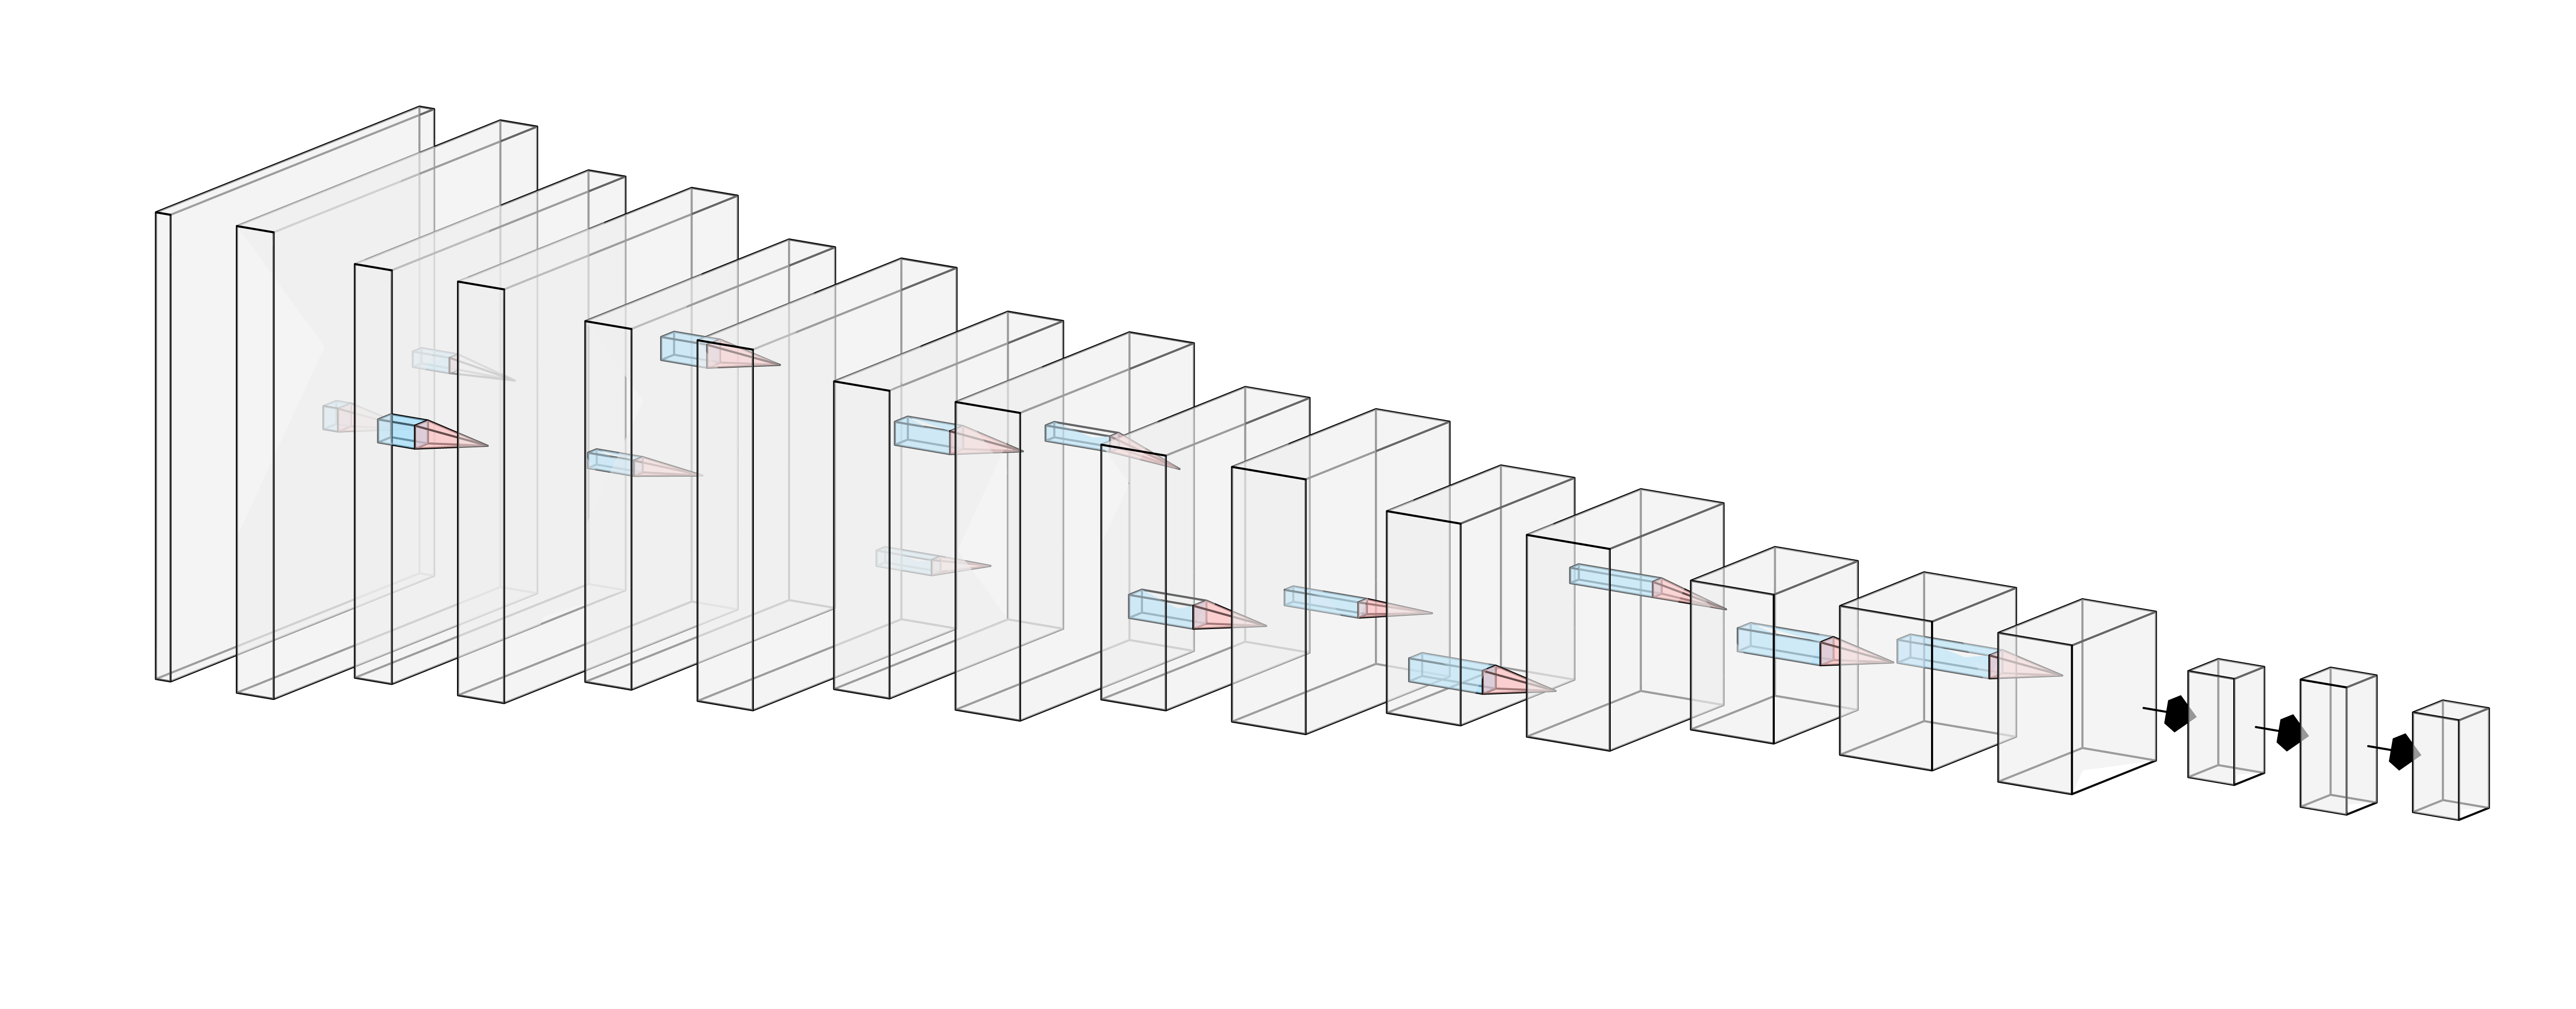
\includegraphics[width=\textwidth]{nn}
\end{figure}

The dimensions of each layer are determined by that of the layer before $N_n$, the kernel size $K$ and the stride length $S$.

\begin{equation}
N_n = \frac{N_{n-1} - K}{S} + 1
\end{equation}

As such, the dimensions for each layer along with filter sizes are listed below.  Layer \texttt{images} is the input layer. All layers beginning with \texttt{conv} are convolutional, layers beginning with \texttt{maxpool} are max pooling layers, and layers beginning with \texttt{fc} are fully connected layers. Interestingly, Tiny YOLOv1 has a unique structure for its output layer. Instead of a rank one tensor for binary classification, YOLOv1 encodes its output in form \texttt{[batchsize, sx, sy, B * (C + 4)]}, where B is number of bounding boxes per grid cell and C is number of classes.

\begin{table}[h!]
\centering
\begin{tabular}{|l|l|l|l|l|}
\hline
Layer    & Output Dimensions  & Filter Size & Stride     & Depth        \\ \hline
images   & {[}448, 448, 3{]}  & -           & -          & -            \\ \hline
conv1    & {[}448, 448, 16{]} & {[}3, 3{]}  & {[}1, 1{]} & 16           \\ \hline
maxpool1 & {[}224, 224, 16{]} & {[}2, 2{]}  & {[}2, 2{]} & -            \\ \hline
conv2    & {[}224, 224, 32{]} & {[}3, 3{]}  & {[}1, 1{]} & 32           \\ \hline
maxpool2 & {[}112, 112, 32{]} & {[}2, 2{]}  & {[}2, 2{]} & -            \\ \hline
conv3    & {[}112, 112, 64{]} & {[}3, 3{]}  & {[}1, 1{]} & 64           \\ \hline
maxpool3 & {[}56, 56, 64{]}   & {[}2, 2{]}  & {[}2, 2{]} & -            \\ \hline
conv4    & {[}56, 56, 128{]}  & {[}3, 3{]}  & {[}1, 1{]} & 128          \\ \hline
maxpool4 & {[}28, 28, 256{]}  & {[}2, 2{]}  & {[}2, 2{]} & -            \\ \hline
conv5    & {[}28, 28, 256{]}  & {[}3, 3{]}  & {[}1, 1{]} & 256          \\ \hline
maxpool5 & {[}14, 14, 256{]}  & {[}2, 2{]}  & {[}2, 2{]} & -            \\ \hline
conv6    & {[}14, 14, 512{]}  & {[}3, 3{]}  & {[}1, 1{]} & 512          \\ \hline
maxpool6 & {[}7, 7, 512{]}    & {[}2, 2{]}  & {[}2, 2{]} & -            \\ \hline
conv7    & {[}7, 7, 1024{]}   & {[}3, 3{]}  & {[}1, 1{]} & 1024         \\ \hline
conv8    & {[}7, 7, 256{]}    & {[}3, 3{]}  & {[}1, 1{]} & 256          \\ \hline
conv9    & {[}7, 7, 512{]}    & {[}3, 3{]}  & {[}1, 1{]} & 512          \\ \hline
fc1      & {[}1024{]}         & -           & -          & -1 (flatten) \\ \hline
fc2      & {[}4096{]}         & -           & -          & -            \\ \hline
fc3      & {[}675{]}          & -           & -          & -            \\ \hline
\end{tabular}
\caption{DetectionNet Architecture}
\end{table}

As seen above, the Tiny YOLOv1 architecture is a simple convolutional network. As a result, we can optimize it with a typical gradient descent optimizer or one of its variants. We opted for an AdamOptimizer with $\alpha = 1\mathrm{e}{-3}$ and $\epsilon = 1.0$, where $\alpha$ represents the learning rate and $\epsilon$ is a constant that is inversely proportional to the size of the weight updates. This function is called to optimized the below cost function.

\begin{equation}
loss = \lambda_{obj}(loss_{dims} + loss_{objconf}  + loss_{prob}) + \lambda_{noobj}(loss_{noobjconf})
\end{equation}

We define two constants that help to correct the unbalance between obj and no\_obj boxes, $\lambda_{obj}$ and $\lambda_{noobj}$. We set these to \textit{5.0} and \textit{0.5} respectively. Additionally, we define $\phi$ as a function that asks like a boolean mask, returning $0$ if the object is in that cell and has that bounding box responsible for its prediction and $1$ otherwise.

\begin{equation}
\phi_{i,j,h}^{obj} =
\begin{cases}
0 & \text{if object is in cell \textit{i,j} and bounding box \textit{h} is responsible} \\
1 & \text{otherwise}
\end{cases}
\end{equation}

We define a few variables for the formulas below. $s_x$ and $s_y$ are defined as number of horizontal grid cells and vertical grid cells respectively. $classes$ is the list of total possible classes. $B$ is the number of bounding boxes per grid cell. $\delta$ is defined as a small constant to prevent extremely small numbers. Then, we define the individual terms in the loss function. $loss_{dims}$ is the sum of the squared errors of the x,y,w,h values of bounding boxes for all squares and bounding boxes responsible.

\begin{equation}
loss_{dims} = \sum\limits_{i=0}^{s_x}\sum\limits_{j=0}^{s_y}\sum\limits_{h=0}^{B}\phi_{i,j,h}^{obj}[(x_{i,j} - \hat{x}_{i,j})^2 + (y_{i,j} - \hat{y}_{i,j})^2 + (\sqrt{w_{i,j} + \delta} - \sqrt{\hat{w_{i,j}} + \delta})^2 + (\sqrt{h_{i,j} + \delta} - \sqrt{\hat{h_{i,j}} + \delta})^2]
\end{equation}

$loss_{objconf}$ is the sum of the squared errors in predicted confidences of all bounding boxes with objects

\begin{equation}
loss_{objconf} = \sum\limits_{i=0}^{s_x}\sum\limits_{j=0}^{s_y}\sum\limits_{h=0}^{B}\phi_{i,j,h}^{obj}(conf_{i,j} - \hat{conf}_{i,j})^2
\end{equation}

$loss_{noobjconf}$ is the sum of the squared errors in predicted confidences of all grid cells with no objects

\begin{equation}
loss_{noobjconf} = \sum\limits_{i=0}^{s_x}\sum\limits_{j=0}^{s_y}\sum\limits_{h=0}^{B}\phi_{i,j,h}^{noobj}(conf_{i,j} - \hat{conf}_{i,j})^2
\end{equation}

$loss_{prob}$ is the sum of the squared errors in predicted class probabilities across all grid cells

\begin{equation}
loss_{prob} = \sum\limits_{i=0}^{s_x}\sum\limits_{j=0}^{s_y}\sum\limits_{c\in classes}^{}\phi_{i,j,h}^{obj}(p(c)_{i,j} - \hat{p(c)}_{i,j})^2
\end{equation}

We also batch normalize every convolutional layer and fully connected layer before activations. This reduces the internal covariate shift, decreasing the time for convergence. In addition, we use a leaky rectified linear unit (ReLU) with an $\alpha = 0.1$. We then define some other parameters for training the network.

\begin{itemize}
  \item $s_x$, $s_y$ = [7, 7]
  \item Batchsize = 16
  \item $B$ = 3
  \item $C$ = 4
  \item Batch Normalization Momentum = 0.9
  \item Batch Normalization $\epsilon$ = 1e-5
\end{itemize}

\subsubsection{Data Cleanup}
Interestingly, KITTI has images that are extremely wide, ranging from [1224, 370] to [1242, 375]. As a result, we need to do additional preprocessing before they are usable.

\paragraph{Images}
\begin{itemize}
    \item Resizing all images to uniform size of [1242, 375] with cubic interpolation
    \item Crop randomly to [375, 375]
    \item Normalize RGB to range [0., 1.]
    \item Pad image size to [448, 448]
\end{itemize}
Resizing then cropping allows us to attain a size closer to 1:1 which is recommended with CNNs with square kernels. We then normalize the color data to ensure that the scale of input remains constant.

\paragraph{Labels}
In the dataset, labels are kept within annotation files. Data is stored in 15 separate columns listed as follows.
\begin{enumerate}
    \item Class - Car, Van, Truck, Pedestrian, Person Sitting, Cyclist, \item Tram, Misc., Don't Care
    \item Boolean, if the bounding box is truncated (leaves the screen)
    \item Boolean, if the bounding box/class is partially obscured
    \item Observation angle - Range from -$\pi$ to $\pi$
    \item Bounding box $x min$ coordinate
    \item Bounding box $y min$ coordinate
    \item Bounding box $x max$ coordinate
    \item Bounding box $y max$ coordinate
    \item 3D - $x$ dimension of object
    \item 3D - $y$ dimension of object
    \item 3D - $z$ dimension of object
    \item x location
    \item y location
    \item z location
    \item ry rotation around y-axis
\end{enumerate}

As we are only concerned with classes and bounding boxes, only columns 1,5,6,7,8 will be used. We then process the labels as follows.

\begin{itemize}
    \item Discard all labels that are not Car / Pedestrian / Cyclist / Misc. Vehicle (Truck or Van)
    \item Discard all labels outside crop range
    \item One-hot encode labels
    \item Convert $p1, p2$ to $x, y, w, h$
    \item Assign boxes to cells
    \item Normalize $w, h$ to cell dimensions
    \item Normalize $x, y$ to image dimensions
    \item Append $obj$, $noobj$, $objI$ boolean masks
\end{itemize}

First, we discard all labels that we are not interested in. Then, as we crop the image, we discard all labels outside that crop range. Then, the labels are one hot encoded to normalize cost. We convert coordinates from form $p1, p2$ (which encodes the $x, y$ coordinates of the top left and bottom right corners of each bounding box) to form $x, y, w, h$ (which encodes the $x, y$ coordinates of the center of the box as well as the height and the width). Each label is then assigned a grid cell, effectively normalizing $x, y, w, h$ to the dimensions of each cell. Boolean masks are then generated depending on whether the grid cell has an object of not.

\subsubsection{Navigation Network}
This part is still very much under construction. This algorithm would be responsible for controlling the actual path of the drones. We plan to create a decentralized autopilot with a Deep Q-Neural Network which is a form of reinforcement learning. We propose the input to be of form \texttt{[$n, r, \phi, \theta$]} where n is number of total drones, r is distance away in pixels, phi is azimuth angle, and theta is elevation angle. We assume $r$ to be infinity when out of range. The goal of the algorithm is to cover the area in the smallest time possible while maintaining communication distance. As a result, the cost function should be affected by total flight time and integral of the distance between drones. Currently, we plan on using a long-short term memory cell (LSTM) networks with the outputs being the velocity deltas in the shape of \texttt{[$n, dx, dy, dz$]}, however, other architectures are being evaluted as well.

\end{document}
